\documentclass[a4paper]{article}
\usepackage{amsfonts}
\usepackage{amsmath}
\usepackage{amssymb}
\usepackage{graphicx}     

\begin{document}
  
\noindent \large Auteur: Stan Van Campenhout \\
\noindent \large Studierichting:  Informatica\\
\noindent \large Oefeningenreeks 3H nr. 9.1\\

\medskip

\normalsize

$ r = 1 + 2\sin\theta $\\

$ \operatorname{dom} = \mathbb{R} $\\

$ p = 2\pi $\\

$ \rightarrow \operatorname{BD} = [0 , 2\pi] $\\

$ r = 0 \Leftrightarrow 2\sin\theta = -1 \Leftrightarrow \sin\theta = -\dfrac{1}{2} \Leftrightarrow \theta = \dfrac{7\pi}{6} + k\pi, \dfrac{11\pi}{6} + k\pi, \forall k \in \mathbb{Z} $\\

$ \rightarrow \left\{\dfrac{7\pi}{6}, \dfrac{11\pi}{6}\right\} $\\

$ r' = 0 \Leftrightarrow 2\cos\theta = 0 \Leftrightarrow \theta = \dfrac{\pi}{2} + k\pi, \forall k \in \mathbb{Z} $\\

$ \rightarrow \left\{\dfrac{\pi}{2}, \dfrac{2\pi}{2}\right\} $\\

\begin{tabular}{ l | c c c c c c c c c c r }	
  $\theta$ &$0$ & &$\dfrac{\pi}{2}$ & &$\dfrac{7\pi}{6}$ & &$\dfrac{3\pi}{2}$ & &$\dfrac{11\pi}{6}$ & &$2\pi$\\ \hline
  $r$ &$+$ &$+$ &$+$ &$+$ &$0$ &$-$ &$-$ &$-$ &$0$ &$+$ &$+$\\
  $r'$ &$+$ &$+$ &$0$ &$-$ &$-$ &$-$ &$0$ &$+$ &$+$ &$+$ &$+$\\ \hline
  $r$ &$\nearrow$ &$\nearrow$ &$M$ &$\searrow$ &$\searrow$ &$\searrow$ &$m$ &$\nearrow$ &$\nearrow$ &$\nearrow$ &$\nearrow$\\
    & & &$3$ & & & &$-1$ & & & &\\
\end{tabular}

\begin{figure}[h]
\centering
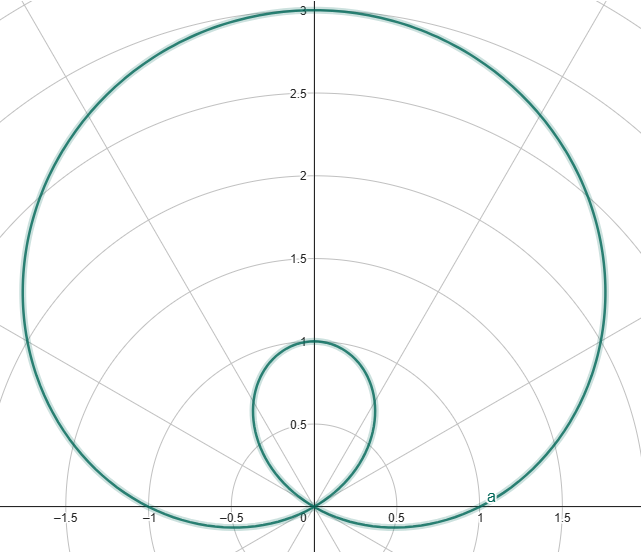
\includegraphics[width=7cm]{3H-9.1-stan.van.campenhout.INF.png}
\end{figure}

\begin{thebibliography}{999}
%\bibitem{a} Referentie
\end{thebibliography}
\end{document} 
